\chapter{狄拉克海、費米子質量與四分量旋量}

\section{右行費米子與狄拉克海}

狄拉克方程是費米子所滿足的方程。相對論性玻色子則滿足不同的方程，例如克萊因--戈登方程或馬克士威方程組。最簡單的例子存在於一維空間，最初描述只能向右運動的粒子與反粒子。

從平面波出發，
\begin{equation}
\psi(x,t)=\psi_0 e^{i(kx-\omega t)}.
\end{equation}
其相速度為
\begin{equation}
v_{\mathrm{ph}}=\frac{\omega}{k}.
\end{equation}
\(k\)和\(\omega\)的正負號很重要。若兩者同號，相位便向右移動；若兩者異號，相位便向左移動。當\(\omega\)與\(k\)成正比時，相速度與群速度相同：
\begin{equation}
v_{\mathrm{g}}=\frac{d\omega}{dk}=\frac{\omega}{k}.
\end{equation}

考慮一階方程
\begin{equation}
\frac{\partial\psi}{\partial x}
+
\frac{\partial\psi}{\partial t}
=0.
\end{equation}
將平面波代入可得
\begin{equation}
ik\psi-i\omega\psi=0,
\end{equation}
因此
\begin{equation}
\omega=k.
\end{equation}
所以這個波向右移動。相應地將這個場標記為下式，是很方便的做法：
\begin{equation}
\frac{\partial\psi_R}{\partial t}
=
-\frac{\partial\psi_R}{\partial x}.
\end{equation}

恢復光速後，有量綱的形式為
\begin{equation}
\frac{\partial\psi_R}{\partial x}
+
\frac{1}{c}\frac{\partial\psi_R}{\partial t}
=0,
\end{equation}
因此
\begin{equation}
\omega=ck.
\end{equation}
以下都令\(c=1\)。在\(\hbar=1\)的單位制中，\(\omega\)也就是一個量子的能量。

\begin{figure}[htbp]
\centering
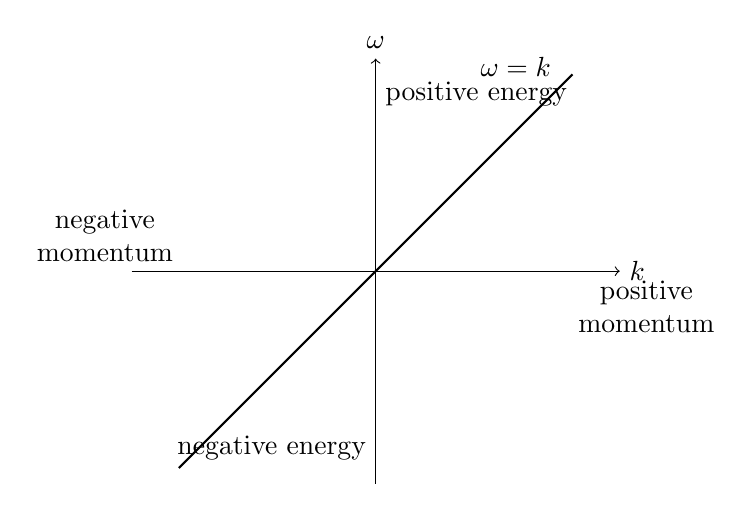
\begin{tikzpicture}[scale=1.0]
\draw[->] (-3.1,0) -- (3.1,0) node[right] {$k$};
\draw[->] (0,-2.7) -- (0,2.7) node[above] {$\omega$};
\draw[thick] (-2.5,-2.5) -- (2.5,2.5);
\node[above left] at (2.35,2.35) {$\omega=k$};
\node[below right,align=center] at (2.45,0) {positive\\momentum};
\node[above left,align=center] at (-2.45,0) {negative\\momentum};
\node[right] at (0,2.25) {positive energy};
\node[left] at (0,-2.25) {negative energy};
\end{tikzpicture}
\caption{無質量右行粒子的色散關係\(\omega=k\)包含正能量支與負能量支。}
\end{figure}

這條直線帶來一個嚴重的後果。\(k\)為正時，能量為正；\(k\)為負時，能量為負。然而兩部分描述的都是向右移動的波，因為整條直線上都有\(\omega/k=1\)。

位於正能量支上的電子可以躍遷到較低的狀態，放出正能量光子，接著再往下躍遷，不斷沿著能譜下行：下一階、再下一階，接著又一階。如此一來，沒有任何電子能保持穩定。更嚴重的是，世界會藉由產生愈來愈多負能量電子來降低能量。

費米子的不相容原理提供了解決辦法：將所有負能量電子態都填滿。已被佔據的態不能再容納另一個電子，因此完全填滿的負能量區域能阻止無止盡的下墜。這個填滿的區域稱為狄拉克海；完全填滿的狀態則是基態，也就是真空。

\begin{classroomqa}
\lecturetimestamp{00:07:19}
\audiencequestion{更低的負能量態有無窮多個嗎？}
\lecturerresponse{有。動量離散時，能譜就像一座無限長的階梯；動量連續時，則像一條連續的滑坡。填滿負能量海可避免電子無止盡地下墜；不過，只要有尚未佔據的較低能態，仍可能發生有限的向下躍遷並放出光子。}
\end{classroomqa}

這說明了為什麼具有這種能譜的方程必須量子化為費米子理論。若量子是玻色子，任意多個玻色子都能佔據同一個較低能態，填滿負能量區域也就無法使真空穩定。

填滿能海的圖像也能說明反粒子的由來。真空中，所有負能量態都已佔據，所有正能量態則為空。電子可以從任一已佔據的負能量態躍遷到任一未佔據的正能量態；初態與末態的能階不必對稱分布。

\begin{figure}[htbp]
\centering
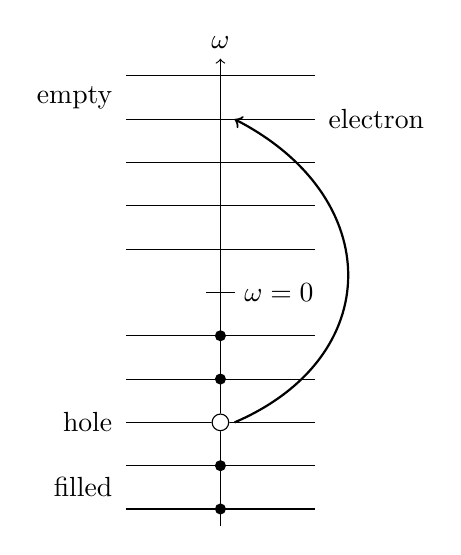
\begin{tikzpicture}[x=1cm,y=0.55cm]
\draw[->] (0,-5.4) -- (0,5.4) node[above] {$\omega$};
\draw (-0.18,0) -- (0.18,0) node[right] {$\omega=0$};
\foreach \y in {-5,-4,-3,-2,-1} {
  \draw (-1.2,\y) -- (1.2,\y);
  \fill (0,\y) circle (2pt);
}
\foreach \y in {1,2,3,4,5} {
  \draw (-1.2,\y) -- (1.2,\y);
}
\draw[->,thick] (0.18,-3) .. controls (2.1,-1.5) and (2.1,2.2) .. (0.18,4);
\draw[white,fill=white] (0,-3) circle (3pt);
\draw (0,-3) circle (3pt);
\node[left] at (-1.25,-3) {hole};
\node[left] at (-1.25,-4.5) {filled};
\node[left] at (-1.25,4.5) {empty};
\node[right] at (1.25,4) {electron};
\end{tikzpicture}
\caption{將已佔據的負能量電子態中的電子躍遷到正能量態，會產生一個正能量電子，並在填滿的能海中留下一個空穴。}
\end{figure}

移除一個負能量電子會使能量相對於真空升高，因此空穴具有正能量。在\(\omega=k\)這一支上，被移除的電子也具有負動量。移除負動量後會留下正的動量盈餘，因此空穴具有正動量。若電子的電荷為負，缺少的電子便對應正電荷。因此，空穴是具有正能量與正動量的反粒子；躍遷後的電子則帶負電荷、具有正能量與正動量。在這個只有一支的理論中，所有真實激發都向右移動。

場\(\psi_R\)由費米子產生與湮滅算符構成。因此，粒子與空穴的詮釋，說的是這個場所產生與移除的量子，而不只是經典波的性質。

不過，這裡仍有不對稱之處。右行能海包含負動量的負能量態，其形式上的總動量極大，方向朝左。可以透過減去這個常數，將真空動量定義為零；但這個狀態在結構上仍不平衡：粒子與反粒子只能向右移動，填滿真空的卻是負動量態。

\section{左行支與平衡的真空}

要平衡左右方向，還需要一個獨立的第二個場，並為它引入自己的產生與湮滅算符。令它滿足
\begin{equation}
\frac{\partial\psi_L}{\partial t}
=
+\frac{\partial\psi_L}{\partial x}.
\end{equation}
對同樣形式的平面波，
\begin{equation}
-i\omega\psi_L=ik\psi_L,
\end{equation}
因此
\begin{equation}
\omega=-k.
\end{equation}
這第二條直線是\(\omega=k\)的鏡像。它的正能量支描述向左移動的粒子，負能量支也必須填滿。

\begin{figure}[htbp]
\centering
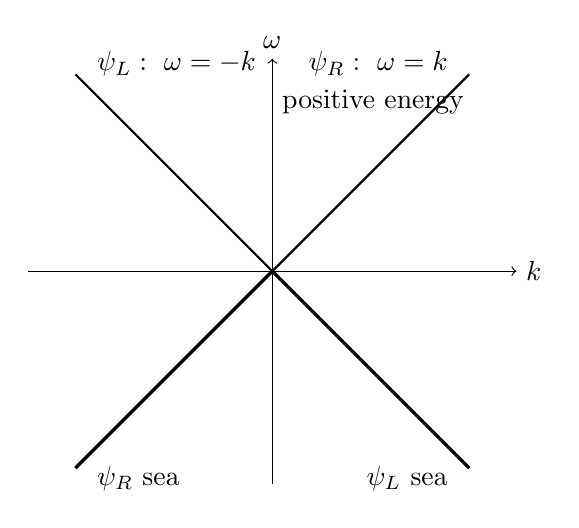
\begin{tikzpicture}[scale=1.0]
\draw[->] (-3.1,0) -- (3.1,0) node[right] {$k$};
\draw[->] (0,-2.7) -- (0,2.7) node[above] {$\omega$};
\draw[thick] (-2.5,-2.5) -- (2.5,2.5);
\draw[thick] (-2.5,2.5) -- (2.5,-2.5);
\draw[very thick] (-2.5,-2.5) -- (0,0);
\draw[very thick] (0,0) -- (2.5,-2.5);
\node[above left] at (2.35,2.35) {$\psi_R:\ \omega=k$};
\node[above right] at (-2.35,2.35) {$\psi_L:\ \omega=-k$};
\node[right] at (0,2.15) {positive energy};
\node[below right] at (-2.35,-2.35) {$\psi_R$ sea};
\node[below left] at (2.35,-2.35) {$\psi_L$ sea};
\end{tikzpicture}
\caption{彼此獨立的右行場與左行場，形成互為鏡像的無質量分支；真空中填滿了兩個負能量半支。}
\end{figure}

填滿兩個負能量海後，向左與向右的已佔據態數量相同，真空中的動量也彼此平衡。粒子與空穴激發現在都可以向任一方向移動。

\begin{classroomqa}
\lecturetimestamp{00:15:58}
\audiencequestion{能否不預設有填滿的態與空穴，也能處理負能量問題？}
\lecturerresponse{同一個理論也可以用另一種方式標記：把已填滿的負能量電子態稱為空的反粒子態。如此一來，物理描述中就只有正能量粒子與反粒子。填滿能海的圖像仍可用來檢查理論的一致性，類似金屬中的填滿能帶：移除電子會留下空穴，而電子躍遷則會同時產生一個粒子與一個空穴。}
\end{classroomqa}

目前討論的激發都是無質量的。它們的色散關係是線性的，速度量值為\(1\)，因此以光速移動。接下來的問題是如何賦予它們質量。

\section{二分量與質量項}

先將兩個場合併寫成一個欄向量：
\begin{equation}
\Psi=
\begin{pmatrix}
\psi_R\\
\psi_L
\end{pmatrix}.
\end{equation}
起初，這只是將兩個獨立方程簡潔地寫在一起。定義
\begin{equation}
\alpha=
\begin{pmatrix}
1&0\\
0&-1
\end{pmatrix}.
\end{equation}
則右行與左行方程可寫成
\begin{equation}
\frac{\partial\Psi}{\partial t}
=
-\alpha\frac{\partial\Psi}{\partial x}.
\end{equation}

\begin{figure}[htbp]
\centering
\includegraphics[width=0.78\textwidth]{lecture_06_figure_02.png}
\caption{場\(\psi_R\)與\(\psi_L\)構成二分量旋量，\(\alpha\)則用來區分兩個無質量分支。}
\lectureframe{00:20:36}
\end{figure}

對平面波而言，算符
\begin{equation}
i\partial_t
\quad\hbox{and}\quad
-i\partial_x
\end{equation}
分別給出\(\omega\)與\(k\)。因此，矩陣方程可簡寫為
\begin{equation}
\omega=\alpha k.
\end{equation}
對上分量而言，這表示\(\omega=k\)；對下分量而言，則表示\(\omega=-k\)。這種記法將兩個方程合併書寫，並未引入新的物理內容。

電子並非無質量，也不以光速移動。一個看似合理的能量公式是非相對論動能\(k^2/(2m)\)，但這不能作為此處的起點：無質量極限所描述的已是以光速移動的情況。相對論關係為
\begin{equation}
\omega^2=k^2+m^2,
\end{equation}
若包含正、負兩個能量支，則為
\begin{equation}
\omega=\pm\sqrt{k^2+m^2}.
\end{equation}
當\(m=0\)時，兩者分別化為\(\omega=k\)與\(\omega=-k\)。

\begin{classroomqa}
\lecturetimestamp{00:25:23}
\audiencequestion{這裡使用的是\(c=1\)的單位制嗎？有質量粒子的速度如何求得？}
\lecturerresponse{是。波包的速度就是群速度；在正能量支上，\(v_{\mathrm g}=d\omega/dk=k/\sqrt{k^2+m^2}\)。因此，色散關係本身就呈現了有質量粒子的速度如何低於\(c=1\)。}
\end{classroomqa}

\begin{classroomqa}
\lecturetimestamp{00:26:29}
\audiencequestion{在簡寫式\(\omega=\alpha k\)中，\(\omega\)是向量還是矩陣？}
\lecturerresponse{這個簡寫代表作用於二分量波函數的算符方程。此處的\(\omega\)表示\(i\partial_t\)，\(k\)表示\(-i\partial_x\)，而\(\alpha\)是作用於分量指標的矩陣。符號\(\omega\)和\(k\)本身是純量；只有在平面波上，它們才取相應的數值本徵值。}
\end{classroomqa}

保留一階方程，並嘗試最簡單的含質量項延伸：
\begin{equation}
\omega=\alpha k+\beta m.
\end{equation}
\(\beta\)必須是矩陣，因為它和\(\alpha\)一樣作用於同一個二分量場。將方程平方，可得它們必須滿足的代數關係：
\begin{align}
\omega^2
&=(\alpha k+\beta m)(\alpha k+\beta m)\\
&=\alpha^2k^2+\beta^2m^2
+\alpha\beta\,km+\beta\alpha\,mk\\
&=\alpha^2k^2+\beta^2m^2
+(\alpha\beta+\beta\alpha)km.
\end{align}
為了對任意\(k\)與\(m\)都得到\(k^2+m^2\)，必須要求
\begin{equation}
\alpha^2=I,
\qquad
\beta^2=I,
\qquad
\alpha\beta+\beta\alpha=0.
\end{equation}

兩個普通的非零數無法滿足最後一個條件：若它們是數，就會得到\(2\alpha\beta=0\)，這與兩者的平方都等於\(1\)矛盾。矩陣則可以反對易。特別是，\(\beta\)不能等於\(\alpha\)，否則
\begin{equation}
\alpha\beta+\beta\alpha=2\alpha^2=2I.
\end{equation}

取
\begin{equation}
\beta=
\begin{pmatrix}
0&1\\
1&0
\end{pmatrix}.
\end{equation}
逐項計算即可檢查它的平方：
\begin{equation}
\begin{aligned}
\beta^2
&=
\begin{pmatrix}
0&1\\
1&0
\end{pmatrix}
\begin{pmatrix}
0&1\\
1&0
\end{pmatrix}\\
&=
\begin{pmatrix}
0\cdot0+1\cdot1&0\cdot1+1\cdot0\\
1\cdot0+0\cdot1&1\cdot1+0\cdot0
\end{pmatrix}
=
\begin{pmatrix}
1&0\\
0&1
\end{pmatrix}.
\end{aligned}
\end{equation}
矩陣相乘的順序很重要：
\begin{align}
\alpha\beta
&=
\begin{pmatrix}
1&0\\
0&-1
\end{pmatrix}
\begin{pmatrix}
0&1\\
1&0
\end{pmatrix}
=
\begin{pmatrix}
0&1\\
-1&0
\end{pmatrix},\\
\beta\alpha
&=
\begin{pmatrix}
0&1\\
1&0
\end{pmatrix}
\begin{pmatrix}
1&0\\
0&-1
\end{pmatrix}
=
\begin{pmatrix}
0&-1\\
1&0
\end{pmatrix}.
\end{align}
因此
\begin{equation}
\alpha\beta=-\beta\alpha,
\qquad
\alpha\beta+\beta\alpha=0.
\end{equation}
也可以選擇其他等價的矩陣；不過這個選擇能讓分量方程特別清楚。

恢復微分算符後，得到有質量的方程
\begin{equation}
i\frac{\partial\Psi}{\partial t}
=
-i\alpha\frac{\partial\Psi}{\partial x}
+m\beta\Psi.
\end{equation}
矩陣\(\beta\)會互換兩個分量：
\begin{equation}
\beta
\begin{pmatrix}
\psi_R\\
\psi_L
\end{pmatrix}
=
\begin{pmatrix}
\psi_L\\
\psi_R
\end{pmatrix}.
\end{equation}
因此，分量方程為
\begin{align}
i\dot{\psi}_R
&=-i\frac{\partial\psi_R}{\partial x}+m\psi_L,\\
i\dot{\psi}_L
&=+i\frac{\partial\psi_L}{\partial x}+m\psi_R.
\end{align}

質量項耦合了無質量理論中原本彼此獨立的場。上分量的方程包含下分量，下分量的方程也包含上分量。這種耦合就是狄拉克質量的意義。這些方程具有平移不變性，因此動量守恆；粒子激發的質量為\(m\)。

\begin{classroomqa}
\lecturetimestamp{00:38:25}
\audiencequestion{一個解會自動具有洛倫茲不變性嗎？}
\lecturerresponse{特定的解不應在洛倫茲變換下保持不變。具有某一動量的狀態會被變換成具有變換後動量的狀態，因此適當的說法是「協變」。關係式\(\omega^2=k^2+m^2\)是檢驗洛倫茲不變性的關鍵之一，但要完整具備協變性，還必須知道旋量\(\Psi\)如何變換；這一點目前尚未建立。}
\end{classroomqa}

\section{靜止系與分量的意義}

無質量粒子無法被帶到靜止系，有質量粒子則可以。在靜止系中\(k=0\)，因此波函數沒有空間變化，且
\begin{equation}
\omega=\beta m.
\end{equation}
微分方程化為
\begin{equation}
i\frac{d\Psi}{dt}=m\beta\Psi.
\end{equation}
寫成分量形式為
\begin{align}
i\dot{\psi}_R&=m\psi_L,\\
i\dot{\psi}_L&=m\psi_R.
\end{align}
\(\beta\)的兩個非對角元素都是\(+1\)，因此這兩個方程都沒有額外的負號。

將兩個分量相加與相減，方程便會解耦。定義
\begin{equation}
\psi_+=\psi_R+\psi_L,
\qquad
\psi_-=\psi_R-\psi_L.
\end{equation}
將兩個靜止系方程相加，得到
\begin{equation}
i\dot{\psi}_+=m\psi_+,
\end{equation}
相減則得到
\begin{equation}
i\dot{\psi}_-=-m\psi_-.
\end{equation}
因此
\begin{equation}
\omega=+m
\quad\hbox{for }\psi_+,
\qquad
\omega=-m
\quad\hbox{for }\psi_-.
\end{equation}

\begin{figure}[htbp]
\centering
\includegraphics[width=0.62\textwidth]{lecture_06_figure_03.png}
\caption{在動量為零時，\(\psi_+=\psi_R+\psi_L\)與\(\psi_-=\psi_R-\psi_L\)的靜止頻率分別為\(\omega=+m\)與\(\omega=-m\)。}
\lectureframe{00:44:49}
\end{figure}

正能量的靜止場為\(\psi_+\)；負能量的靜止場為\(\psi_-\)。和先前一樣，負能量態都已填滿。靜止系中的結果只是完整能譜在\(k=0\)處的切片：
\begin{equation}
\omega_\pm(k)=\pm\sqrt{k^2+m^2}.
\end{equation}
\begin{figure}[htbp]
\centering
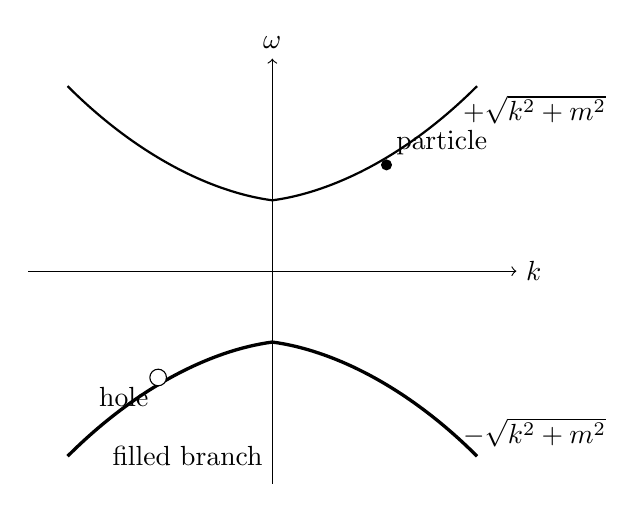
\begin{tikzpicture}[scale=1.0]
\draw[->] (-3.1,0) -- (3.1,0) node[right] {$k$};
\draw[->] (0,-2.7) -- (0,2.7) node[above] {$\omega$};
\draw[thick] (-2.6,2.35)
  .. controls (-1.7,1.45) and (-0.75,1.0) .. (0,0.9)
  .. controls (0.75,1.0) and (1.7,1.45) .. (2.6,2.35);
\draw[very thick] (-2.6,-2.35)
  .. controls (-1.7,-1.45) and (-0.75,-1.0) .. (0,-0.9)
  .. controls (0.75,-1.0) and (1.7,-1.45) .. (2.6,-2.35);
\fill (1.45,1.35) circle (2pt);
\node[above right] at (1.45,1.35) {particle};
\fill[white] (-1.45,-1.35) circle (3pt);
\draw (-1.45,-1.35) circle (3pt);
\node[below left] at (-1.45,-1.35) {hole};
\node[right] at (2.3,2.05) {$+\sqrt{k^2+m^2}$};
\node[right] at (2.3,-2.05) {$-\sqrt{k^2+m^2}$};
\node[left] at (0,-2.35) {filled branch};
\end{tikzpicture}
\caption{每一個動量值都有正能量態與負能量態。負能量支已填滿，其中缺失的態便是具有正能量的空穴。}
\end{figure}
每個動量值都對應一個正能量態與一個負能量態。填滿負能量支的所有態後，能海上方留下正能量粒子，海中則留下正能量空穴。粒子與空穴的質量都為正。

這個要點值得再說一次：費米子的兩個分量原本彼此獨立，耦合之後便帶有質量。在靜止系中，原來的任一分量單獨都不是能量本徵態；具有確定能量的態是兩個分量的和與差。

要理解這個和的意義，可將相關的單粒子產生部分記作\(C_R^\dagger\)與\(C_L^\dagger\)。作用於真空時，
\begin{equation}
(C_R^\dagger+C_L^\dagger)\lvert0\rangle
\end{equation}
會產生一個處於兩個分量相干疊加態的粒子，而不是兩個粒子。若寫成乘積，
\begin{equation}
C_R^\dagger C_L^\dagger\lvert0\rangle,
\end{equation}
就含有兩個產生算符；兩個模式都可用時，這會產生一個雙粒子態。歸一化後，靜止態出現在兩個分量中的機率相等，但耦合後的整個波函數動量為零。

只有在\(m=0\)時，標記\(R\)與\(L\)才直接表示運動方向。加入質量項後，運動中的有質量解通常同時包含兩個分量；靜止解中兩者的振幅大小也相等。因此，此處最好把\(R\)與\(L\)視為旋量上分量和下分量的標記。

\begin{figure}[htbp]
\centering
\includegraphics[width=0.78\textwidth]{lecture_06_figure_04.png}
\caption{質量不為零時，兩個旋量分量彼此耦合；只有在無質量極限下，才能直接將它們詮釋為右行與左行分量。}
\lectureframe{00:50:48}
\end{figure}

粒子物理學中的所有有質量費米子，都由左分量場與右分量場構成：狄拉克質量會耦合無質量極限下彼此獨立的分量。

\begin{classroomqa}
\lecturetimestamp{00:52:01}
\audiencequestion{\(\psi_R\pm\psi_L\)是否應包含\(1/\sqrt{2}\)這個因子？}
\lecturerresponse{可以加入這個因子來歸一化狀態。它會同時乘在方程兩側，因此不會改變運動方程。}
\end{classroomqa}

\begin{classroomqa}
\lecturetimestamp{00:52:12}
\audiencequestion{右分量與左分量的相對大小重要嗎？}
\lecturerresponse{在所選的靜止系本徵態中，兩者的振幅大小相等。整體歸一化可任意選擇，但相對大小由\(\beta\)的本徵向量決定。}
\end{classroomqa}

\begin{classroomqa}
\lecturetimestamp{00:52:52}
\audiencequestion{兩個分量之間可以有相對相位嗎？}
\lecturerresponse{可以。\(\psi_R\pm\psi_L\)中的實係數，是採用實矩陣\(\beta\)的結果。其他平方等於單位矩陣且與\(\alpha\)反對易的矩陣，也都是等價選擇；在這些選擇下，分量之間可能會出現相位。選定一種表示後，就必須前後一致地使用。}
\end{classroomqa}

\begin{classroomqa}
\lecturetimestamp{00:53:43}
\audiencequestion{加入質量後，``左行波''和``右行波''這些標籤會不會造成誤解？}
\lecturerresponse{多少會。這些標籤在無質量理論中，確實描述向左與向右移動的波。質量不為零時，即使粒子沿單一方向移動，通常也同時包含兩個分量，因此用``上分量''與``下分量''稱呼會比較恰當。}
\end{classroomqa}

\begin{classroomqa}
\lecturetimestamp{00:55:01}
\audiencequestion{靜止的費米子是否已經需要自旋角動量？}
\lecturerresponse{在這個一維模型中不需要。角動量在一維空間中沒有定義，因此目前的建構尚未涉及自旋。}
\end{classroomqa}

\begin{classroomqa}
\lecturetimestamp{00:55:24}
\audiencequestion{波函數是否包含費米子的產生與湮滅算符？}
\lecturerresponse{是。}
\end{classroomqa}

\begin{classroomqa}
\lecturetimestamp{00:55:30}
\audiencequestion{除了選用產生與湮滅算符之外，費米子特性還體現在哪裡？}
\lecturerresponse{費米子的產生--湮滅規則也體現了這一特性。具有這種負能量能譜的方程，必須依照這些規則量子化；若採用玻色子的佔據規則，真空就會不穩定。相對論性玻色子必須用不同的波動方程描述。}
\end{classroomqa}

\begin{classroomqa}
\lecturetimestamp{00:56:20}
\audiencequestion{非零動量的解能否經洛倫茲變換成靜止系的解？}
\lecturerresponse{可以。洛倫茲推進可以將有質量的解變換到其靜止系；不過，實際進行變換時，必須知道洛倫茲變換如何作用於旋量\(\Psi\)。}
\end{classroomqa}

\section{標量真空場如何產生質量}

\begin{classroomqa}
\lecturetimestamp{00:58:11}
\audiencequestion{與希格斯場的交互作用如何產生狄拉克質量項？}
\lecturerresponse{將常數質量係數換成與標量場的耦合。若該場在真空中為零，費米子就仍然無質量；若該場在真空中具有固定的非零值，這項耦合的作用便完全等同於質量。}
\end{classroomqa}

令\(\phi(x,t)\)為具有自身運動方程的標量場。在狄拉克方程的質量項中，將常數\(m\)換成\(g\phi(x,t)\)：\footnote{將先前建立的質量項\(m\beta\Psi\)作此替換，就得到所示的交互作用項。}
\begin{equation}
i\frac{\partial\Psi}{\partial t}
=
-i\alpha\frac{\partial\Psi}{\partial x}
+g\phi(x,t)\,\beta\Psi.
\end{equation}
於是兩個場方程便彼此耦合。費米子會作用於標量場，標量場也會反過來作用於費米子；整體來看，這個系統是非線性的，儘管在\(\phi\)給定時，狄拉克方程對\(\Psi\)而言是線性的。

先假設空無一物的空間中
\begin{equation}
\phi(x,t)=0.
\end{equation}
如此一來，混合項消失，上、下分量彼此解耦，費米子也就沒有質量。反之，若最低能量態中的標量場為固定的非零值，
\begin{equation}
\phi(x,t)=\phi_0\neq0.
\end{equation}
該真空中的狄拉克方程便成為
\begin{equation}
i\frac{\partial\Psi}{\partial t}
=
-i\alpha\frac{\partial\Psi}{\partial x}
+g\phi_0\,\beta\Psi,
\end{equation}
因此
\begin{equation}
m_{\mathrm{eff}}=g\phi_0.
\end{equation}
所以，玻色場與費米場的耦合，加上空無一物的空間中玻色場的非零值，會產生左右分量間的混合；這和先前直接寫入方程的質量項所造成的混合相同。

\begin{classroomqa}
\lecturetimestamp{01:01:27}
\audiencequestion{LHC能否提供真空中存在非零希格斯場的證據？}
\lecturerresponse{當然可以。這是重大議題之一。}
\end{classroomqa}

\begin{classroomqa}
\lecturetimestamp{01:01:32}
\audiencequestion{可以再說明希格斯機制如何運作嗎？}
\lecturerresponse{標量場在空間與時間中的變化會帶有能量，也可能具有局域勢能\(V(\phi)\)。若勢能的極小值出現在\(\phi\)的非零值處，真空中便會有非零場。將場在選定極小值附近的振盪量子化，就得到希格斯粒子。}
\end{classroomqa}

場可透過兩種不同方式攜帶能量。有一部分能量取決於場在空間與時間中如何變化。熟悉的例子是馬克士威場：
\begin{equation}
\mathcal{E}_{\mathrm{Maxwell}}\propto \mathbf E^2+\mathbf B^2,
\end{equation}
\(\mathbf E\)與\(\mathbf B\)都由電磁勢的導數構成。因此，這部分能量與底層場在空間與時間中的變化有關。

標量場也可以有局域勢能密度，
\begin{equation}
V(\phi),
\end{equation}
它取決於\(\phi\)本身的值，而非其導數。概略來說，
\begin{equation}
\mathcal{E}_\phi
=
\mathcal E_{\text{space and time gradients}}+V(\phi).
\end{equation}
若沒有更深層的原理加以限定，\(V(\phi)\)可以是任何符合模型對稱性的合理函數。

在此處採用的簡化實純量場例子中，令理論在
\begin{equation}
\phi\longrightarrow-\phi.
\end{equation}
之下保持對稱。因此，勢能必須是偶函數：
\begin{equation}
V(\phi)=V(-\phi).
\end{equation}
這個對稱性本身並未指出極小值的位置。一種可能是在\(\phi=0\)處有唯一的極小值；另一種可能是在非零值處有兩個對稱的極小值，一正一負。

\begin{figure}[htbp]
\centering
\includegraphics[width=0.72\textwidth]{lecture_06_figure_05.png}
\caption{極小值位於\(\phi=0\)時，真空場為零；若存在對稱的非零極小值，真空場便可取值\(\phi_0\neq0\)，從而產生費米子質量\(g\phi_0\)。}
\lectureframe{01:04:47}
\end{figure}

不必指定勢能的具體多項式形式，也能畫出這兩種可能性。\footnote{下方曲線只呈現論證所需的定性特徵：一種是中心極小值，另一種是彼此對稱的極小值。}
\begin{figure}[htbp]
\centering
\resizebox{\linewidth}{!}{%
\begin{tikzpicture}[x=1.35cm,y=1.05cm]
\begin{scope}[shift={(-3.1,0)}]
\draw[->] (-1.7,0) -- (1.7,0) node[right] {$\phi$};
\draw[->] (0,-0.15) -- (0,2.45) node[above] {$V(\phi)$};
\draw[thick] (-1.5,2.05) .. controls (-0.9,0.65) and (-0.45,0.25) .. (0,0.25)
             .. controls (0.45,0.25) and (0.9,0.65) .. (1.5,2.05);
\fill (0,0.25) circle (1.2pt);
\node[below] at (0,0) {$0$};
\end{scope}
\begin{scope}[shift={(3.1,0)}]
\draw[->] (-1.7,0) -- (1.7,0) node[right] {$\phi$};
\draw[->] (0,-0.15) -- (0,2.45) node[above] {$V(\phi)$};
\draw[thick] (-1.55,2.05)
  .. controls (-1.25,0.75) and (-1.0,0.25) .. (-0.75,0.25)
  .. controls (-0.35,0.25) and (-0.25,1.3) .. (0,1.3)
  .. controls (0.25,1.3) and (0.35,0.25) .. (0.75,0.25)
  .. controls (1.0,0.25) and (1.25,0.75) .. (1.55,2.05);
\fill (-0.75,0.25) circle (1.2pt);
\fill (0.75,0.25) circle (1.2pt);
\node[below] at (0,0) {$0$};
\node[below] at (-0.75,0) {$-\phi_0$};
\node[below] at (0.75,0) {$\phi_0$};
\end{scope}
\end{tikzpicture}%
}
\caption{偶勢能可以有位於中心的極小值，也可以有兩個彼此對稱的非零極小值。}
\end{figure}

若極小值位於原點，真空便有\(\phi_0=0\)，這項耦合不會使電子具有質量。若極小值位於\(\phi=\pm\phi_0\)，真空便會落在其中一個極小值。兩種選擇由對稱性相互關聯，而且無論選哪一個，都會在狄拉克方程中產生非零係數\(g\phi_0\)。至於勢能為什麼具有這種定性形狀，是更深一層的問題，單靠這個機制無法解答。

場不必恰好停在極小值處，也可以像粒子在勢阱底部附近那樣，繞著選定值振盪。將這些振盪量子化，就得到希格斯量子。其特徵頻率與希格斯粒子的質量有關：質量愈大，激發單一量子所需的能量也愈大。在真空中，場只是在極小值附近保持穩定，並提供費米子質量。場一旦振動，這種振動便是希格斯粒子。

這種耦合包含作用與反作用。費米子會對\(\phi\)的值產生反應；能量足夠高的費米子碰撞也能激發標量場。碰撞必須提供激發所需的能量；場開始振動後，其量子就是希格斯粒子。同一個場不只與電子耦合，也與夸克場及其他由它提供質量的場耦合。

\begin{classroomqa}
\lecturetimestamp{01:08:14}
\audiencequestion{希格斯場振動或偏離真空值時，電子質量會改變嗎？}
\lecturerresponse{會。有效質量與場的局域值成正比，因此場偏向零值時，質量會降低。若要讓一個宏觀區域長時間維持在遠離真空值的狀態，需要極大的能量；足以進行這種實驗的區域可能會坍縮成黑洞。}
\end{classroomqa}

這個思想實驗很直接。若能讓某個區域維持在\(\phi=0\)附近，則該區域內的
\begin{equation}
m_{\mathrm{eff}}=g\phi
\end{equation}
會變小或消失。受激的希格斯模態會繞著真空值振盪；但若要在整個宏觀區域造成並維持顯著位移，就需要極大的能量。勢能代價會隨體積增加。在這樣的區域成為實際可用的實驗室之前，其能量就可能已足以造成引力坍縮。質量原則上確實會改變，但要實現大幅且可觀測的變化極其困難。

\begin{classroomqa}
\lecturetimestamp{01:09:27}
\audiencequestion{為什麼需要希格斯場？}
\lecturerresponse{因為電子具有質量。}
\end{classroomqa}

\begin{classroomqa}
\lecturetimestamp{01:09:41}
\audiencequestion{每種粒子都各自有一個希格斯場嗎？}
\lecturerresponse{不是。在標準模型中，同一個希格斯場為電子、夸克及參與這項機制的其他粒子提供質量。超對稱版本需要兩個希格斯場，而不是為每種粒子各設一個場。}
\end{classroomqa}

單一場的圖像只是示意：完整的希格斯場比單一實數\(\phi\)包含更多結構。儘管如此，核心概念仍然成立。同一個真空場可以用不同的耦合強度與不同費米子作用，因此，不同粒子具有不同質量，並不表示每種粒子都需要各自的希格斯場。希格斯粒子就是同一個場繞著真空值振盪所形成的粒子。

為什麼不直接把電子質量寫進方程，而不引入希格斯場？這與弱交互作用及統一有關，留待後續討論。

\begin{classroomqa}
\lecturetimestamp{01:11:16}
\audiencequestion{超對稱理論中是否有兩個希格斯場部門？}
\lecturerresponse{是。在此處採用的簡化劃分中，一個為上型夸克提供質量，另一個則為下型夸克與電子提供質量。這種數量加倍是超對稱性的技術要求，並非每種粒子各有一個希格斯場。}
\end{classroomqa}

\begin{classroomqa}
\lecturetimestamp{01:12:01}
\audiencequestion{如果希格斯粒子有質量，那麼它的質量從何而來？}
\lecturerresponse{這裡尚未解答這個問題。更值得追問的是，為什麼希格斯粒子的質量如此小。}
\end{classroomqa}

對稱性與質量問題密不可分。在簡單的狄拉克模型中，若某種對稱性禁止左、右兩個部分混合，混合項的係數就必須為零。若真空態保有這種對稱性，費米子便會是無質量的。非零的希格斯真空值會破壞相關的真空對稱性，使左右耦合成為可能：
\begin{equation}
m_{\mathrm{eff}}=g\phi_0\neq0.
\end{equation}
此處不推導確切的對稱變換，重點在於它對質量項的影響。方程或許具有這種對稱性，但特定的最低能量態未必如此。提供質量的正是這種真空的不對稱性。

在此勾勒的電弱理論圖像中，電子和夸克以這種方式獲得質量，\(W\) 和 \(Z\) 玻色子也是如此。光子則保持無質量。希格斯粒子本身是另一個例外：即使沒有相同的真空位移，它也可以有質量；它的質量涉及自身場的振盪，而非左右費米子的混合。因此，在這套論述中，希格斯真空值使其他粒子獲得質量；至於希格斯激發本身的質量，則是另一個問題。

\begin{classroomqa}
\lecturetimestamp{01:15:26}
\audiencequestion{引力子有質量嗎？}
\lecturerresponse{沒有。引力子和光子一樣是無質量的。過去人們也曾認為中微子沒有質量，但中微子其實有極小的質量；用這裡的說法，就是它們的左、右分量之間只有極微弱的耦合。}
\end{classroomqa}

光子以及理論中的引力子都是無質量的，並以光速運動。中微子則不完全屬於這一類。在狄拉克的語言中，中微子的微小質量表示連結其左、右分量的耦合極微弱。這種耦合為何如此微弱，是另一個問題。

\section{三維空間中的狄拉克方程}

在三維空間中，波數成為波向量，
\begin{equation}
\mathbf{k}=(k_1,k_2,k_3),
\end{equation}
其分量分別沿著 \(x\)、\(y\) 和 \(z\) 方向。一維關係的形式為
\begin{equation}
\omega=\alpha k+\beta m,
\end{equation}
最簡單的線性推廣則是
\begin{equation}
\omega
=
\alpha_1 k_1+\alpha_2 k_2+\alpha_3 k_3+\beta m.
\end{equation}
此處的 \(\alpha_i\) 和 \(\beta\) 是矩陣，必須選得滿足
\begin{equation}
\omega^2=k_1^2+k_2^2+k_3^2+m^2.
\end{equation}
這個不變的色散關係是必要條件，但單靠它還不足以涵蓋相對論的全部內容。

將線性表示式平方可得
\begin{align}
\omega^2
={}&
\alpha_1^2k_1^2+\alpha_2^2k_2^2+\alpha_3^2k_3^2+\beta^2m^2
\nonumber\\
&+(\alpha_1\alpha_2+\alpha_2\alpha_1)k_1k_2
+(\alpha_1\alpha_3+\alpha_3\alpha_1)k_1k_3
\nonumber\\
&+(\alpha_2\alpha_3+\alpha_3\alpha_2)k_2k_3
+\sum_{i=1}^{3}(\alpha_i\beta+\beta\alpha_i)k_i m.
\end{align}
平方動量項與質量項的係數必須滿足
\begin{equation}
\alpha_1^2=\alpha_2^2=\alpha_3^2=I,
\qquad
\beta^2=I.
\end{equation}
若不同的 \(\alpha\) 矩陣彼此反對易，不需要的 \(k_i k_j\) 項便會消失：
\begin{equation}
\alpha_i\alpha_j+\alpha_j\alpha_i=0,
\qquad i\neq j.
\end{equation}
若滿足下式，混合的 \(k_i m\) 項便會消失：
\begin{equation}
\alpha_i\beta+\beta\alpha_i=0
\qquad
\text{for each }i.
\end{equation}
因此，四個矩陣的平方都等於單位矩陣，而且任意兩個不同的矩陣都彼此反對易。

確實存在三個具有所需相互反對易性質的 \(2\times2\) 矩陣，也就是三個泡利矩陣。不存在第四個 \(2\times2\) 矩陣，能同時滿足平方等於單位矩陣並與這三個矩陣全部反對易。\(3\times3\) 矩陣也無法實現這些條件。最小可行的表示使用 \(4\times4\) 矩陣，也就是狄拉克矩陣。

從兩個分量增加到四個分量，帶出了一個物理問題。在一維空間的例子中，兩個分量起初分別是向右和向左傳播的場。那麼四個分量代表什麼？新增的要素是自旋；但自旋涉及角動量，因此必須在真正的三維空間中討論。

矩陣的選擇並不唯一。不同的選擇彼此等價，就像互相垂直的座標軸有不同選法一樣：矩陣元素會改變，但可透過變換互相轉換，物理內容則不變。一種方便的表示法是\footnote{以下逐項列出的矩陣，是前面所示分塊形式與泡利矩陣的展開；講座在 01:30:23--01:31:29 明確說明了這些分塊關係。}
\begin{equation}
\beta=
\begin{pmatrix}
1&0&0&0\\
0&1&0&0\\
0&0&-1&0\\
0&0&0&-1
\end{pmatrix},
\end{equation}
以及
\begin{align}
\alpha_1&=
\begin{pmatrix}
0&0&0&1\\
0&0&1&0\\
0&1&0&0\\
1&0&0&0
\end{pmatrix},
&
\alpha_2&=
\begin{pmatrix}
0&0&0&-i\\
0&0&i&0\\
0&-i&0&0\\
i&0&0&0
\end{pmatrix},
\\[1ex]
\alpha_3&=
\begin{pmatrix}
0&0&1&0\\
0&0&0&-1\\
1&0&0&0\\
0&-1&0&0
\end{pmatrix}.
\end{align}
將每個矩陣分成 \(2\times2\) 區塊，就更容易看出其結構：
\begin{equation}
\beta=
\begin{pmatrix}
I_2&0\\
0&-I_2
\end{pmatrix},
\qquad
\alpha_i=
\begin{pmatrix}
0&\sigma_i\\
\sigma_i&0
\end{pmatrix}.
\end{equation}
三個泡利矩陣為
\begin{equation}
\sigma_1=
\begin{pmatrix}
0&1\\
1&0
\end{pmatrix},
\quad
\sigma_2=
\begin{pmatrix}
0&-i\\
i&0
\end{pmatrix},
\quad
\sigma_3=
\begin{pmatrix}
1&0\\
0&-1
\end{pmatrix}.
\end{equation}
這些分塊矩陣滿足所需的狄拉克反對易關係。

現在，波函數必須有四個分量：
\begin{equation}
\Psi=
\begin{pmatrix}
\psi_1\\
\psi_2\\
\psi_3\\
\psi_4
\end{pmatrix}.
\end{equation}
運動方程為
\begin{equation}
i\frac{\partial\Psi}{\partial t}
=
-i\sum_{j=1}^{3}\alpha_j
\frac{\partial\Psi}{\partial x_j}
+\beta m\Psi.
\end{equation}
這個簡潔的表示式代表四個彼此耦合的線性微分方程。\(\alpha_j\) 矩陣的非對角元素以比一維情形更複雜的方式混合這四個分量，但基本結構相同：矩陣將各分量耦合起來，而方程對空間和時間的導數仍都是一階。分量數目額外加倍，正是引出自旋的線索。

\begin{classroomqa}
\lecturetimestamp{01:33:53}
\audiencequestion{\(\Psi\) 的四個分量，是直接對應時空四個維度的四維向量嗎？}
\lecturerresponse{不是。它們構成的是旋量，而不是四維向量。一維例子中，時空維度數和旋量分量數恰好同為二，純屬巧合。在更高維的構造中，旋量矩陣的維度是二的冪次，通常不等於時空維度數。}
\end{classroomqa}

靜止系再次提供了最簡單的解釋。動量為零時，導數項消失：
\begin{equation}
i\frac{\partial\Psi}{\partial t}=m\beta\Psi.
\end{equation}
在所選的表示法中，\(\beta\) 有兩個本徵值為 \(+1\)，另外兩個本徵值為 \(-1\)。因此，有兩個能量為 \(+m\) 的靜止態，以及兩個能量為 \(-m\) 的靜止態。和先前一樣，負能態都被填滿。每個能量符號下各有兩個態，這種額外的簡併結構，其物理解釋就是自旋。

\begin{classroomqa}
\lecturetimestamp{01:35:51}
\audiencequestion{\(\alpha_i\) 的非對角區塊應該帶有相同的指標，使它們都是 \(\sigma_i\) 嗎？}
\lecturerresponse{是的。每個 \(\alpha_i\) 矩陣的兩個非對角區塊中，都包含相應的泡利矩陣 \(\sigma_i\)。}
\end{classroomqa}

\begin{classroomqa}
\lecturetimestamp{01:36:03}
\audiencequestion{\(\alpha_i\) 的簡潔反對易關係中，是否漏了一個因子二？}
\lecturerresponse{是的。當 \(i=j\) 時，左側等於 \(\alpha_i^2+\alpha_i^2=2I\)。正確的關係是 \(\alpha_i\alpha_j+\alpha_j\alpha_i=2\delta_{ij}I\)。}
\end{classroomqa}

因此，平方條件與指標不相等時的條件可以合併為
\begin{equation}
\alpha_i\alpha_j+\alpha_j\alpha_i=2\delta_{ij}I.
\end{equation}

\begin{classroomqa}
\lecturetimestamp{01:36:42}
\audiencequestion{狄拉克的構造中，改用四個矩陣是否是重大的概念飛躍？}
\lecturerresponse{是的。狄拉克假設了這個方程，再追究它的推論。一項推論是反粒子的出現，另一項是自旋。自旋早已從實驗中得知，但這個方程說明了它。}
\end{classroomqa}

\begin{classroomqa}
\lecturetimestamp{01:37:29}
\audiencequestion{是先有實驗證據，還是先有將粒子限制為玻色子或費米子的定理？}
\lecturerresponse{實驗證據先出現，定理則是後來才提出。玻色子--費米子的二分法適用於三個空間維度。在兩個空間維度加上一個時間維度時，可能出現中間統計；在 \(3+1\) 維以及更高的空間維度中，可能的統計則只有玻色子和費米子兩種。}
\end{classroomqa}

\begin{classroomqa}
\lecturetimestamp{01:39:01}
\audiencequestion{\(\Psi\) 的四個分量有慣用的指標嗎？}
\lecturerresponse{此處並未固定某種必要的選法。可以用 \(p\) 和 \(q\) 作為標記，取值從一到四；如此一來，每個矩陣就各有一個行指標和一個列指標。}
\end{classroomqa}

矩陣記號會省略這些分量標記。若將它們寫出來，則有
\begin{equation}
p,q=1,2,3,4,
\end{equation}
方程可寫成
\begin{equation}
i\,\partial_t\Psi_p
=
-i\sum_{j=1}^{3}\sum_{q=1}^{4}
(\alpha_j)_{pq}\,\partial_j\Psi_q
+m\sum_{q=1}^{4}\beta_{pq}\Psi_q.
\end{equation}

\begin{classroomqa}
\lecturetimestamp{01:40:15}
\audiencequestion{使用矩陣乘法時，分量指標就不必明寫了嗎？}
\lecturerresponse{是的。矩陣記號會自動省略這些指標。之後還可以引入一種更對稱的形式，讓相對論結構更加明顯。}
\end{classroomqa}

展示的方程是最簡單的 \(3+1\) 維形式的狄拉克方程。接下來要理解自旋，並建立相對論性玻色子的波動方程，因為狄拉克方程並不是描述玻色子的方程，而自然界中約有一半粒子是玻色子。有了這些要素，就能進一步探討夸克、輕子、弱玻色子、希格斯粒子和光子，讓粒子譜更有條理。整個討論還需要更多對稱性。